\section{Systemübersicht und Datenmodel}

\subsection{Systemübersicht}

Für die Erstellung des Systems wurden im Vorfeld die folgenden Anwendungsfälle (Usecases) 
identifiziert und in einem Usecase-Diagramm dokumentiert.\newline


\noindent Es wurde bewusst entschieden, lediglich eine Benutzerrolle zu implementieren, um den 
Verwaltungsaufwand für den Betrieb des Systems möglichst gering zu halten. Da es sich um ein 
kollaboratives Quizsystem handelt, haben alle Benutzer die Möglichkeit, gemeinsam Fragen zu 
erstellen und zu bearbeiten.\newline

\noindent Im folgenden werden die identifizierten Usecases beschrieben.

\begin{figure}[H]
  \centering
  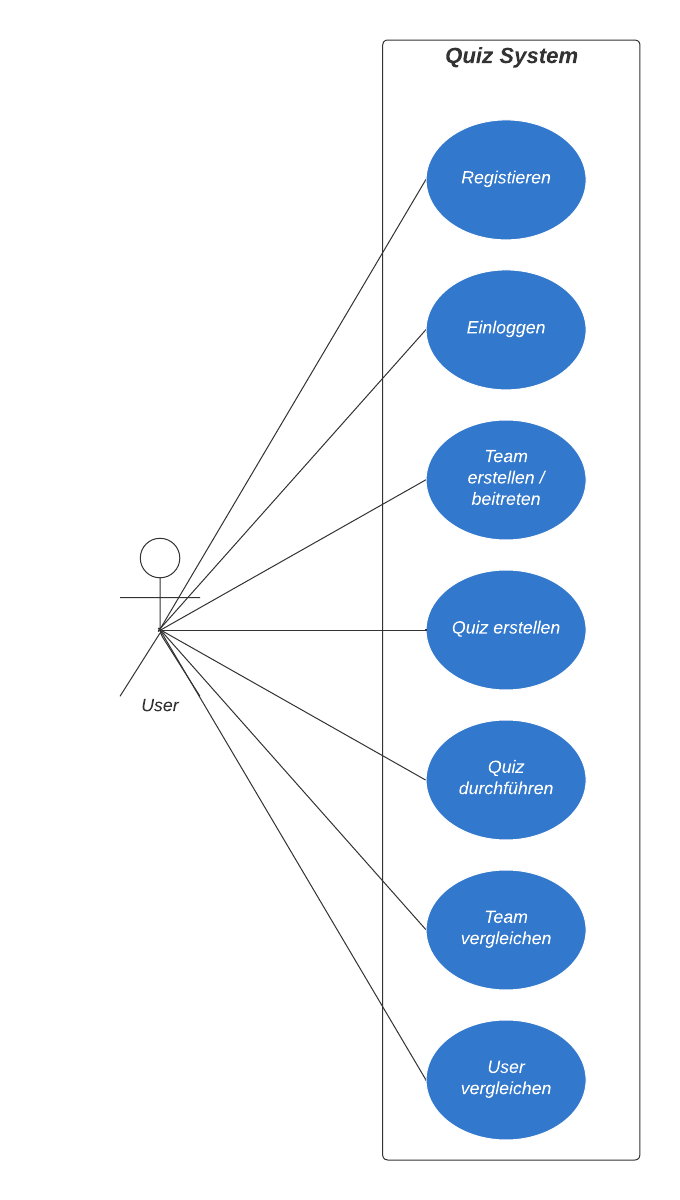
\includegraphics[width=0.5\textwidth]{img/Quiz System - Use Case Diagramm.png}
  \caption{Usecase Diagramm}
\end{figure}

\subsubsection{Usecase: Benutzer Registieren}

Der Use Case 'Benutzer Registieren' beschreibt den Prozess, bei dem ein neuer Benutzer sich in das System einträgt, 
um darauf zugreifen und die Funktionalitäten des Systems nutzen zu können. Die Registrierung ist 
notwendig, um die Identität des Benutzers zu etablieren und ihm die Möglichkeit zu geben, 
personalisierte Aktionen im System durchzuführen. Während des Registrierungsprozesses gibt der 
Benutzer persönliche Informationen an, wie seinen Benutzernamen, eine E-Mail-Adresse und ein 
Passwort. Nachdem die Registrierung erfolgreich abgeschlossen wurde, erhält der Benutzer 
Zugriff auf das System und kann die Funktionalitäten nutzen.

\subsubsection*{Vorbedingungen}

\begin{itemize}
  \item Der Benutzer hat eine aktive Internetverbindung und hat einen Webbrowser installiert.
  \item Das System ist verfügbar und erlaubt Benutzerregistrierungen..
\end{itemize}

\subsubsection*{Erfolgsablauf}

\begin{enumerate}
  \item Der Benutzer navigiert zur Registrierungsseite des Systems.
  \item Der Benutzer gibt die erforderlichen Registrierungsinformationen ein, einschließlich Name, E-Mail-Adresse und Passwort.
  \item Das System validiert die eingegebenen Daten und überprüft, ob die E-Mail-Adresse und der Benutzernamen eindeutig ist und den Anforderungen entspricht.
  \item Das System erstellt ein Benutzerkonto und speichert die Registrierungsinformationen in der Datenbank.
  \item Der Benutzer erhält eine Bestätigung über die erfolgreiche Registrierung und kann sich nun im System anmelden.
\end{enumerate}

\subsubsection*{Alternative Abläufe}

\begin{itemize}
  \item Falls die eingegebenen Informationen unvollständig oder ungültig sind, wird der Benutzer aufgefordert, die Informationen zu korrigieren
   und den Registrierungsvorgang erneut zu starten.
\end{itemize}

\subsubsection*{Nachbedingungen}

\begin{itemize}
  \item Das System hat ein neues Benutzerkonto erstellt und die Registrierungsinformationen in der Datenbank gespeichert.
  \item Der Benutzer kann sich nun mit seinem Benutzernamen und Passwort im System anmelden.
  \item Der Benutzer kann nun die Funktionalitäten des Systems nutzen.
\end{itemize}

\subsubsection{Usecase: Benutzer Anmelden}

Der Use Case 'Benutzer Anmelden' beschreibt den Prozess, bei dem ein bereits registrierter Benutzer sich in das System einloggt,
um Zugriff auf seine personalisierten Funktionen und Daten zu erhalten. Die Anmeldung ermöglicht es dem Benutzer, 
sein Konto zu authentifizieren und sich im System zu identifizieren, um das System vollumfänglich nutzen zu können.

\subsubsection*{Vorbedingungen}

\begin{itemize}
  \item Der Benutzer hat eine aktive Internetverbindung und hat einen Webbrowser installiert.
  \item Der Benutzer hat bereits ein Benutzerkonto im System erstellt.
  \item Das System ist verfügbar und erlaubt Benutzeranmeldungen.
\end{itemize}

\subsubsection*{Erfolgsablauf}

\begin{enumerate}
  \item Der Benutzer befindet sich auf Anmeldeseite des Systems.
  \item Der Benutzer gibt seinen Benutzernamen und sein Passwort ein.
  \item Das System validiert die eingegebenen Daten und überprüft, ob die E-Mail-Adresse und der Benutzernamen eindeutig ist und den Anforderungen entspricht.
  \item Das System authentifiziert den Benutzer und erstellt eine Sitzung.
  \item Der Benutzer erhält eine Bestätigung über die erfolgreiche Anmeldung und kann nun die Funktionalitäten des Systems nutzen.
\end{enumerate}

\subsubsection*{Alternative Abläufe}

\begin{itemize}
  \item Falls die eingegebenen Informationen unvollständig oder ungültig sind, wird der Benutzer aufgefordert, die Informationen zu korrigieren
   und den Anmeldevorgang erneut zu starten.
\end{itemize}

\subsubsection*{Nachbedingungen}

\begin{itemize}
  \item Das System hat eine Sitzung für den Benutzer erstellt.
  \item Der Benutzer kann nun die Funktionalitäten des Systems unter einer Identität nutzen.
\end{itemize}

\subsubsection{Usecase: Team erstellen \& beitretten}

Der Use Case 'Team erstellen \& beitretten' beschreibt den Prozess, bei dem Benutzer Teams erstellen und ihnen beitreten können, um gemeinsam an 
kollaborativen Aktivitäten innerhalb des Systems teilzunehmen. Jeder Benutzer kann einem Team beitreten, wobei nur der Eigentümer (Team Owner) eines 
Teams das Recht hat, das Team zu bearbeiten oder zu löschen.

\subsubsection*{Vorbedingungen}

\begin{itemize}
  \item Der Benutzer hat eine aktive Internetverbindung und hat einen Webbrowser installiert.
  \item Der Benutzer hat sich erfolgreich im System angemeldet.
  \item Das System ist verfügbar und erlaubt das Erstellen und Beitreten von Teams.
\end{itemize}

\subsubsection*{Erfolgsablauf}

\begin{enumerate}
  \item Der Benutzer befindet sich auf der Teamseite des Systems.
  \item Der Benutzer erstellt ein neues Team und gibt einen Namen für das Team ein.
  \item Das System erstellt ein neues Team und speichert die Informationen in der Datenbank.
  \item Der Benutzer erhält eine Bestätigung über die erfolgreiche Erstellung des Teams und kann nun das Team bearbeiten.
  \item Der Benutzer kann dem Team beitreten.
\end{enumerate}

\subsubsection*{Alternative Abläufe}

\begin{itemize}
  \item Falls die eingegebenen Informationen unvollständig oder ungültig sind, wird der Benutzer aufgefordert, die Informationen zu korrigieren
   und den Erstellungsprozess erneut zu starten.
\end{itemize}

\subsubsection*{Nachbedingungen}

\begin{itemize}
  \item Das System hat ein neues Team erstellt und die Informationen in der Datenbank gespeichert.
  \item Der Benutzer kann nun das Team bearbeiten.
  \item Der Benutzer kann dem Team beitreten.
\end{itemize}

\subsubsection{Usecase: Quiz erstellen}

Der Use Case 'Quiz erstellen' beschreibt den Prozess, bei dem Benutzer ein Quiz erstellen können, um es mit anderen Benutzern zu teilen. 
Dabei besteht ein Quiz aus mindestens 10 Fragen, die vom Benutzer erstellt werden müssen bevor das Quiz aufgeführt werden kann. 
Jeder Benutzer kann das Quiz bearbeiten, wobei nur der Eigentümer (Quiz Owner) eines Quiz das Recht hat, das Quiz zu löschen.
Bei der Erstellung einer Frage muss der Benutzer mindestens eine richtige Antwort und eine falsche Antwort angeben.

\subsubsection*{Vorbedingungen}

\begin{itemize}
  \item Der Benutzer hat eine aktive Internetverbindung und hat einen Webbrowser installiert.
  \item Der Benutzer hat sich erfolgreich im System angemeldet.
  \item Das System ist verfügbar und erlaubt das Erstellen von Quiz.
\end{itemize}

\subsubsection*{Erfolgsablauf}

\begin{enumerate}
  \item Der Benutzer befindet sich auf der Quiz-Übserichtsseite des Systems.
  \item Der Benutzer erstellt ein neues Quiz und gibt einen Namen für das Quiz ein.
  \item Das System erstellt ein neues Quiz und speichert die Informationen in der Datenbank.
  \item Der Benutzer erhält eine Bestätigung über die erfolgreiche Erstellung des Quiz und kann nun das Quiz bearbeiten.
  \item Der Benutzer kann dem Quiz Fragen hinzufügen.
\end{enumerate}

\subsubsection*{Alternative Abläufe}

\begin{itemize}
  \item Falls die eingegebenen Informationen unvollständig oder ungültig sind, wird der Benutzer aufgefordert, die Informationen zu korrigieren
   und den Erstellungsprozess erneut zu starten.
\end{itemize}

\subsubsection*{Nachbedingungen}

\begin{itemize}
  \item Das System hat ein neues Quiz erstellt und die Informationen in der Datenbank gespeichert.
  \item Der Benutzer kann nun das Quiz bearbeiten.
  \item Der Benutzer kann dem Quiz Fragen hinzufügen.
  \item Das Quiz kann ab 10 Fragen aufgeführt werden.
\end{itemize}

\subsubsection{Usecase: Quiz durchführen}

Der Use Case 'Quiz durchführen' beschreibt den Prozess, bei dem Benutzer ein Quiz durchführen können, um ihre Kenntnisse zu testen.
Dabei besteht ein Quiz aus mindestens 10 Fragen, weswegen ein Quiz erst gestartet werden kann, wenn es 10 Fragen enhält.
Der Nutzer kann die Quiz-Seite jederzeit verlassen. Der letzte Stand wird immer gespeicher und auf dem Dashboard angezeigt.
Wenn ein Quiz nicht vollumfänglich durchgeführt wurde kann es später fortgesetzt werden.

\subsubsection*{Vorbedingungen}

\begin{itemize}
  \item Der Benutzer hat eine aktive Internetverbindung und hat einen Webbrowser installiert.
  \item Der Benutzer hat sich erfolgreich im System angemeldet.
  \item Das System ist verfügbar und erlaubt das Durchführen von Quiz.
  \item Das Quiz enthält mindestens 10 Fragen.
\end{itemize}

\subsubsection*{Erfolgsablauf}

\begin{enumerate}
  \item Der Benutzer befindet sich auf der Quiz-Übserichtsseite des Systems.
  \item Der Benutzer wählt ein Quiz aus und startet es.
  \item Das System zeigt die eine Frage an und wartet auf die Antwort des Benutzers.
  \item Der Benutzer wählt eine Antwort aus und bestätigt seine Auswahl.
  \item Das Quiz ist beendet und dem User wird eine Übserichtsseite angezeigt.
\end{enumerate}

\subsubsection*{Alternative Abläufe}

\begin{itemize}
  \item Falls die eingegebenen Informationen unvollständig oder ungültig sind, wird der Benutzer aufgefordert, die Informationen zu korrigieren
   und den Erstellungsprozess erneut zu starten.
\end{itemize}

\subsubsection*{Nachbedingungen}

\begin{itemize}
  \item Das System hat die Antworten des Benutzers gespeichert.
  \item Der Benutzer kann das Quiz jederzeit fortsetzen falls es nicht abgeschlossen wurde.
  \item Der erreichte Score des Quiz durchgangs wurde dem User und dem Team des Users gutgeschrieben
\end{itemize}

\subsubsection{Usecase: Teams \& Nutzer vergleichen}

Der Use Case 'Teams \& Nutzer vergleichen' beschreibt den Prozess, bei dem Benutzer ihre Ergebnisse mit anderen Benutzern vergleichen können.
Dazu findet der Nutzer auf seinem Dashboard eine Übersicht über seine Ergebnisse und eine Rangliste der Teams und User. 
Dies soll den Nutzer ermutigen mehr Quizze zu lösen.

\subsubsection*{Vorbedingungen}

\begin{itemize}
  \item Der Benutzer hat eine aktive Internetverbindung und hat einen Webbrowser installiert.
  \item Der Benutzer hat sich erfolgreich im System angemeldet.
  \item Das System ist verfügbar und erlaubt das zugreifen auf das Dashboard.
\end{itemize}

\subsubsection*{Erfolgsablauf}

\begin{enumerate}
  \item Der Benutzer befindet sich auf der Dashboard-Übserichtsseite des Systems.
  \item Der Benutzer sieht seine Ergebnisse und die Rangliste der Teams und User.
\end{enumerate}

\subsection*{Nachbedingungen}

\begin{itemize}
  \item Der Benutzer kann seine Ergebnisse mit anderen Benutzern vergleichen.
  \item Der Benutzer kann seine Ergebnisse mit anderen Teams vergleichen.
\end{itemize}

\subsection{Projektaufbau \& Frameworks}

Unser Projekt besteht aus zwei wesentlichen Komponenten: dem Frontend und dem Backend.\newline

\noindent Das Frontend ist die Schnittstelle, die auf der Client-Seite im Webbrowser ausgeführt wird.
Diese Komponente ist für die Darstellung der Benutzeroberfläche verantwortlich. 
Sie ermöglicht den Benutzern die Interaktion mit dem System, das Einsehen von Inhalten, das 
Durchführen von Aktionen und das Erleben einer reibungslosen Nutzererfahrung. 
Das Frontend bildet die sichtbare und benutzerfreundliche Oberfläche, die es den Benutzern 
ermöglicht, mit dem System zu interagieren.\newline

\noindent Das Backend hingegen operiert auf der Server-Seite und übernimmt Aufgaben im Hintergrund. 
Hier findet die Verarbeitung von Daten, die Verwaltung von Benutzerkonten, die Interaktion mit der 
Datenbank und die Bereitstellung von Informationen für das Frontend statt. 
Das Backend fungiert als das 'Gehirn' des Systems und ermöglicht die reibungslose Ausführung 
aller Systemfunktionen.\newline

\noindent Eine wichtige Unterscheidung zwischen Frontend und Backend ist die Art der Ausführung. 
Während das Frontend clientseitig im Browser des Benutzers läuft, wird das Backend serverseitig 
betrieben. Diese Trennung ermöglicht eine effiziente Aufgabenteilung und sorgt dafür, 
dass die Anforderungen der Benutzer effektiv verarbeitet werden.\newline

\noindent Die Entscheidung, Frontend und Backend getrennt voneinander zu entwickeln, 
wurde bewusst getroffen und bringt mehrere Vorteile mit sich:

\begin{itemize}
  \item \textbf{Unabhängige Entwicklung:} Die beiden Komponenten können unabhängig voneinander 
  entwickelt werden. Dies ermöglicht es, unterschiedliche Teams oder Entwickler für das Frontend 
  und das Backend einzusetzen, was die Effizienz der Entwicklung steigern kann.
  \item \textbf{Unabhängige Tests:} Die beiden Komponenten können unabhängig voneinander getestet 
  werden. Dadurch können Fehler und Probleme frühzeitig erkannt und behoben werden, ohne die 
  gesamte Anwendung zu beeinträchtigen.
  \item \textbf{Unabhängige Bereitstellung (Deployment):} Frontend und Backend können unabhängig 
  voneinander bereitgestellt werden. Updates oder Änderungen in einer Komponente erfordern 
  nicht zwangsläufig, dass die andere ebenfalls angepasst werden muss.
  \item \textbf{Skalierbarkeit:} Jede Komponente kann unabhängig voneinander skaliert werden, 
  um den Anforderungen des Systems und der Benutzer gerecht zu werden. Dies ermöglicht eine 
  effiziente Ressourcennutzung.
\end{itemize}

\noindent Für die Implementierung des Frontends haben wir uns für das Angular-Framework entschieden.
Angular ist ein leistungsstarkes JavaScript-Framework, das die Entwicklung von anspruchsvollen 
Webanwendungen erleichtert. Es bietet eine breite Palette von Tools und Bibliotheken, 
die es Entwicklern ermöglichen, eine benutzerfreundliche Benutzeroberfläche zu erstellen. \newline

\noindent Das Backend wurde mithilfe des ASP.NET Frameworks realisiert. 
ASP.NET ist ein Framework, das sich besonders für die Entwicklung serverseitiger Anwendungen eignet. 
Es bietet eine Vielzahl von Erweiterungen und Tools, die sich hervorragend für die Implementierung 
einer robusten Web-API eignen.\newline

\noindent Als Datenbank haben wir uns für PostgreSQL entschieden. 
PostgreSQL ist eine Open-Source-relationale Datenbank, die im Vergleich zu MySQL den Vorteil bietet, 
keine Lizenzprobleme zu verursachen. Sie ermöglicht die effiziente Speicherung und Verwaltung von 
Daten, die in der Anwendung benötigt werden.\newline

\noindent Die Kommunikation zwischen Frontend und Backend wurde über eine REST-API realisiert. 
Eine REST-API definiert klare Strukturen für die API-Endpunkte, was die Kommunikation zwischen 
den beiden Komponenten vereinfacht. Über diese API-Schnittstelle können Anwendungen Anfragen an 
das Backend senden und Informationen austauschen. Dies ermöglicht eine nahtlose Integration 
von Frontend und Backend.\newline

\noindent Eine bemerkenswerte Stärke dieser Architektur besteht darin, dass sie eine spätere 
Entwicklung einer mobilen App ermöglicht, die die gleichen Funktionalitäten wie die 
Webanwendung bietet, ohne dass Änderungen am Backend-Code erforderlich sind. 
Dies bietet eine flexible Grundlage für die Erweiterung und Weiterentwicklung des Systems.\newline

\begin{figure}[H]
  \centering
  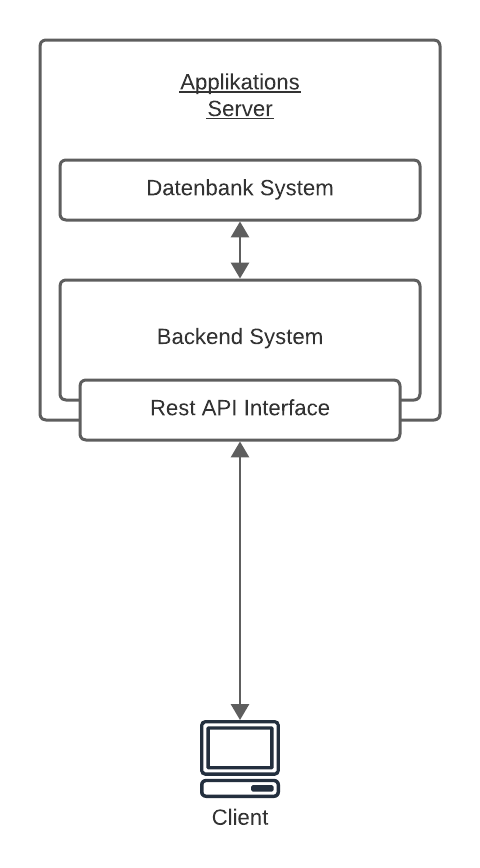
\includegraphics[width=0.5\textwidth]{img/API Kommunikation.png}
  \caption{API Kommunikation}
\end{figure}

\subsection{Datenmodelle}

Die Anwendung enthält 4 verschiedene Datenmodelle die im folgenden beschrieben werden:

\begin{itemize}
  \item \textbf{Frontend Datenmodel:} ie Frontend-Modelle sind Datenmodelle, die ausschließlich im Frontend-Bereich der 
  Anwendung Verwendung finden. Abhängig von der Gestaltung des Frontends können diese Modelle von den API-Modellen abweichen. 
  In solchen Fällen erfolgt die Zuordnung der API-Modelle zu den Frontend-Modellen durch Mapping-Prozesse.
  \item \textbf{Rest-API Datenmodel / DTO Modelle:} REST-API-Modelle, die auch als DTO-Modelle bezeichnet werden, sind Datenmodelle, 
  die im Backend-Bereich der Anwendung Anwendung finden. Sie dienen zur Definition der Schnittstellen der API und werden von der API an 
  das Frontend gesendet. Im Backend-Bereich werden die DTO-Modelle in die Backend-Modelle überführt (gemappt).
  \item \textbf{Backend Modelle:} Backend-Modelle sind Datenmodelle, die ausschließlich im Backend-Bereich der Anwendung Verwendung finden. 
  Sie sind darauf ausgerichtet, die bereitgestellten Funktionen effizient auszuführen. Im Backend-Bereich werden die Backend-Modelle 
  entweder in die Datenbankmodelle überführt (gemappt) oder in die DTO-Modelle überführt (gemappt).
  \item \textbf{Datenbank Modelle:} Datenbank-Modelle sind spezielle Datenmodelle, die ausschließlich im Kontext der Datenbankverwaltung 
  in der Anwendung Verwendung finden. Ihr Hauptzweck besteht darin, Daten effizient zu speichern und zu verwalten. 
  Im Datenbank-Bereich werden diese Datenbank-Modelle vom Backend gelesen und in die Backend-Modelle überführt (gemappt).

  In diesem Projekt nutzen wir das Entity Framework, welches die Datenbank-Modelle automatisch aus den Backend-Modellen generiert. 
  Ebenso erfolgt die automatische Überführung der Datenbank-Modelle in die Backend-Modelle (Mapping). 
  Darüber hinaus ist für das Entity Framework ein sogenannter Lazy Loading Proxy installiert, der Subproperties automatisch dann 
  lädt, wenn sie benötigt werden.
\end{itemize}


\noindent Besondere Aufmerksamkeit verdient die Betrachtung der API-Modelle und Datenbankmodelle, da diese häufig eine gemeinsame Struktur
 mit den Frontend-Modellen aufweisen. Dies geschieht in der Regel, da das Entity Framework die Datenbankmodelle automatisch aus
den Backend-Modellen generiert. \newline

\noindent Im Folgenden werden wir näher auf die Hintergrund-Modelle (Backend Modelle), die API-Modelle und die Datenbankmodelle eingehen:

\subsubsection{Backend Modelle}

Die Backend-Modelle sind die Datenmodelle, die speziell für die Verarbeitung im Backend der Anwendung verwendet werden. 
Sie sind darauf ausgerichtet, die bereitgestellten Funktionen effizient auszuführen und den Prozess möglichst einfach und 
eindeutig abzubilden. In der folgenden Abbiildung werden die Backend-Modelle in einem UML-Diagramm dargestellt.

\begin{figure}[H]
  \centering
  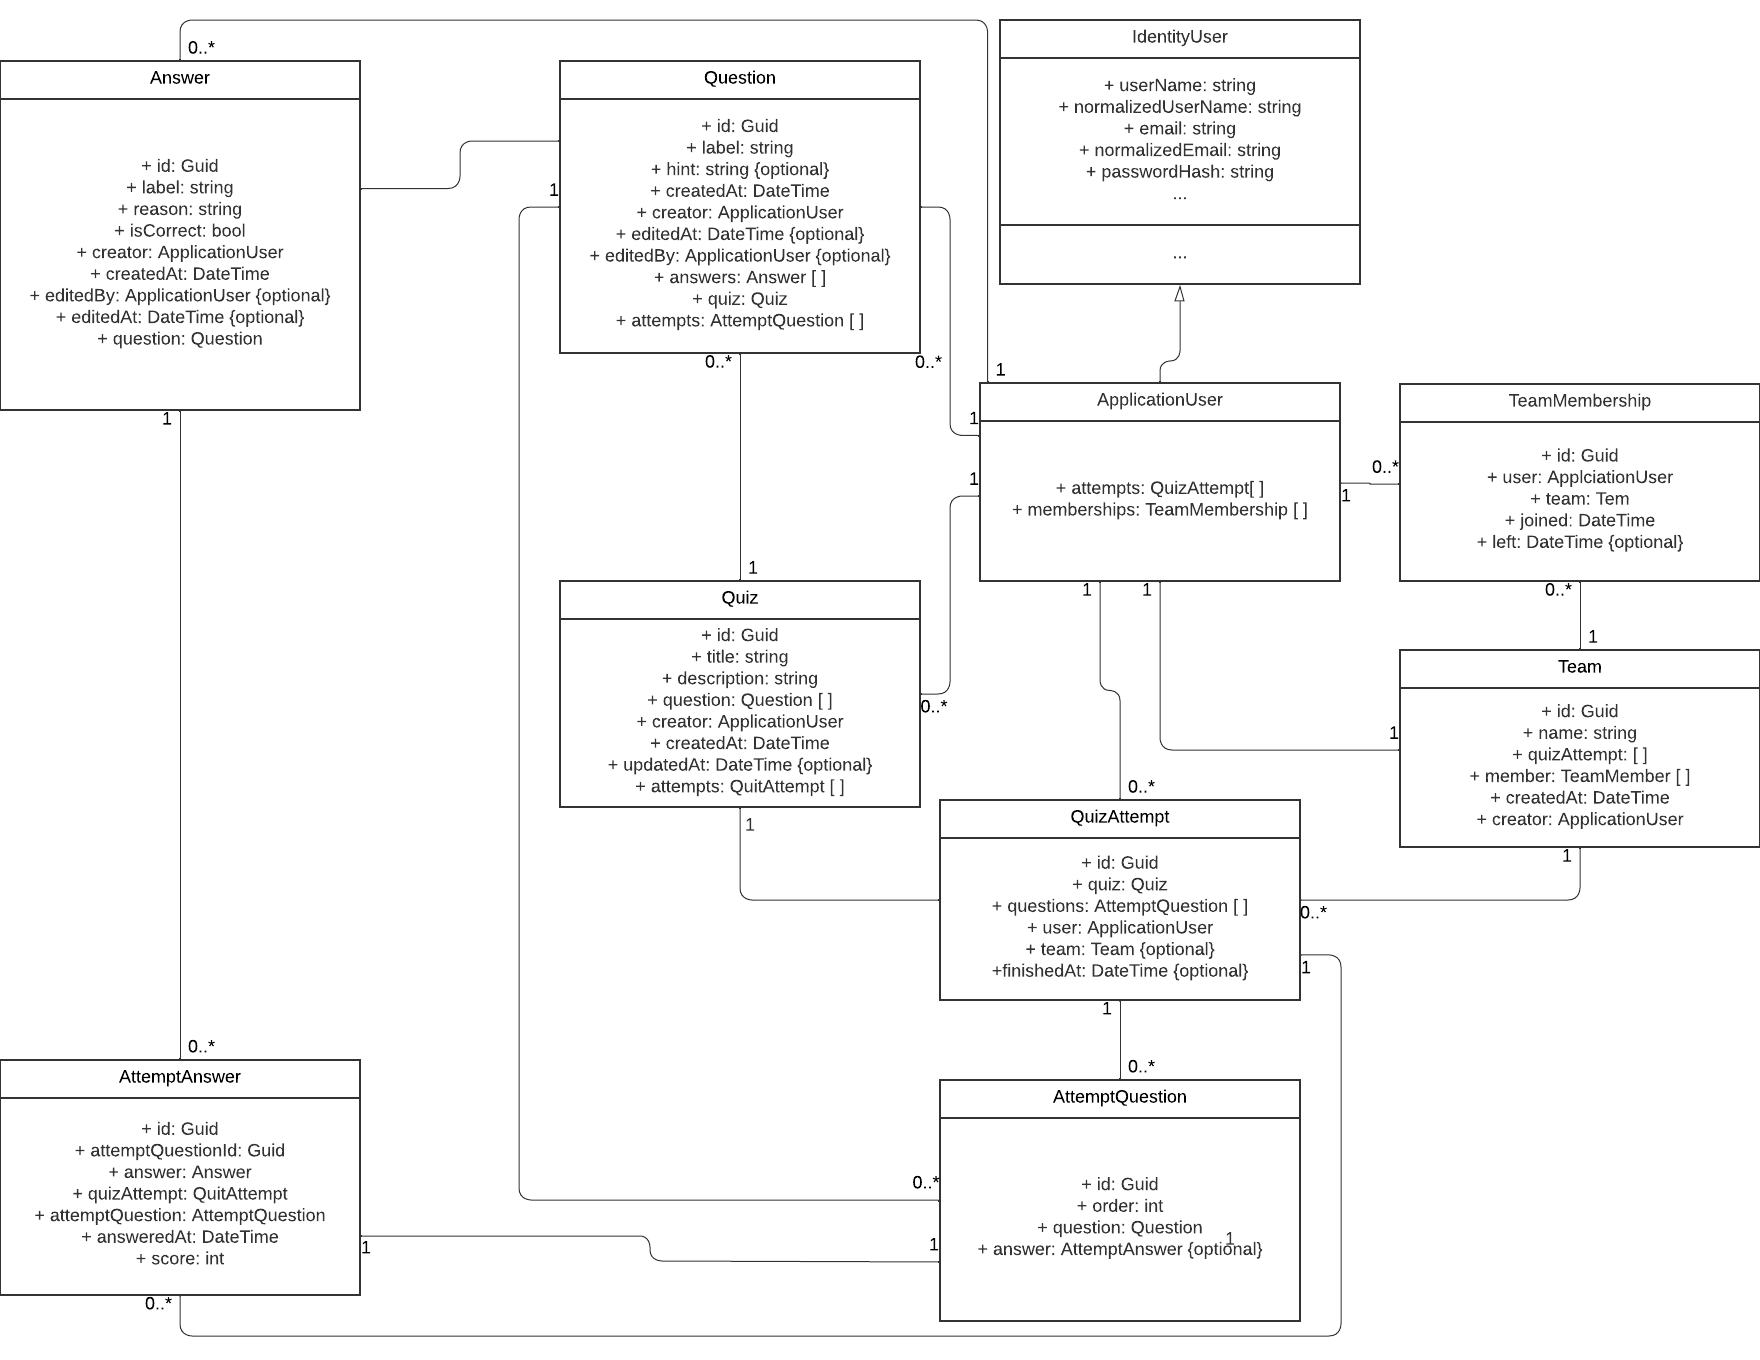
\includegraphics[width=0.5\textwidth]{img/UML-Klasse.png}
  \caption{UML Diagramm der Backend Modelle}
\end{figure}

\noindent Die Backend-Modelle aus dem UML-Diagramm werden im Folgenden näher erläutert:\newline

\noindent\textbf{'ApplicationUser' Klasse:} Im Zentrum der Applikationsmodelle steht die Klasse 'ApplicationUser', die den Benutzer der Anwendung repräsentiert. 
Diese Klasse erbt von der 'IdentityUser' Klasse, die vom ASP.NET Identity Framework bereitgestellt wird. Der ASP.NET Identity Framework 
bietet Funktionen zur Benutzerverwaltung, einschließlich des Anmelde- und Registrierungsprozesses. Darüber hinaus ermöglicht er die 
Verwaltung von Rollen und Ansprüchen (Claims), obwohl diese Funktionen in dieser Applikation nicht genutzt werden. \newline

\noindent\textbf{'Team' Klasse:} Die 'Team'-Klasse repräsentiert ein Team, das von einem Benutzer erstellt werden kann. 
Ein Team kann mehrere Mitglieder haben, und es ist mit dem Quiz-Versuch des Benutzers verknüpft, sofern dieser Mitglied des Teams ist. 
Auf dieser Grundlage kann der Team-Score berechnet werden. \newline

\noindent\textbf{'Quiz' Klasse:} Die 'Quiz'-Klasse repräsentiert ein Quiz, das von einem Benutzer erstellt werden kann. 
Ein Quiz kann mehrere Fragen haben, die in der 'Question'-Klasse abgebildet sind. Zudem ist das Quiz mit dem Quiz-Versuch des Benutzers 
verknüpft, sofern dieser das Quiz erstellt hat. \newline

\noindent\textbf{'Question' Klasse:} Die 'Question'-Klasse repräsentiert eine Frage, die zu einem Quiz gehört. 
Eine Frage kann mehrere Antworten haben, die in der 'Answer'-Klasse abgebildet werden. Zudem ist die Frage mit dem Quiz-Versuch des 
Benutzers verknüpft, sofern dieser die Frage erstellt hat. \newline

\noindent\textbf{'Answer' Klasse:} Die 'Answer'-Klasse repräsentiert eine Antwort, die zu einer Frage gehört. 
Wenn ein Benutzer einen Quiz-Versuch startet, wird für jede Frage eine 'AttemptQuestion'-Instanz erstellt, die mit der 
gewählten Antwort verknüpft wird. Dies ermöglicht die Speicherung der Ergebnisse des Versuchs. \newline

\noindent\textbf{'AttemptQuestion' Klasse:} Die 'AttemptQuestion'-Klasse repräsentiert eine Frage, die zu einem Quiz-Versuch gehört. 
Wenn ein Benutzer einen Quiz-Versuch startet, wird für jede Frage eine 'AttemptQuestion'-Instanz erstellt, die mit der gewählten 
Antwort verknüpft wird. Dies dient zur Erfassung und Speicherung der Ergebnisse des Versuchs. \newline

\noindent\textbf{'QuizAttempt' Klasse:} Die 'QuizAttempt'-Klasse repräsentiert einen Quiz-Versuch, den ein Benutzer starten kann. 
Ein Versuch kann mehrere 'AttemptQuestion'-Instanzen haben, die die Fragen des Versuchs repräsentieren. Zudem ist der 
Versuch mit dem Quiz verknüpft, das der Benutzer versucht hat. \newline

\subsubsection{Datenbank Modelle}

Die Datenbank-Modelle sind spezielle Datenmodelle, die ausschließlich im Kontext der Datenbankverwaltung in der Anwendung Verwendung finden.
In dieser Anwendung werden die Datenbank-Modelle über das Entity Framework automatisch aus den Backend-Modellen generiert. 
Diese Verfahrensweise nennt sich Code-First-Approach. \newline

\noindent Im Folgenden werden die Datenbank-Modelle näher erläutert und in einem Entity Relationship Diagramm (ERD) dargestellt:

\begin{figure}[H]
  \centering
  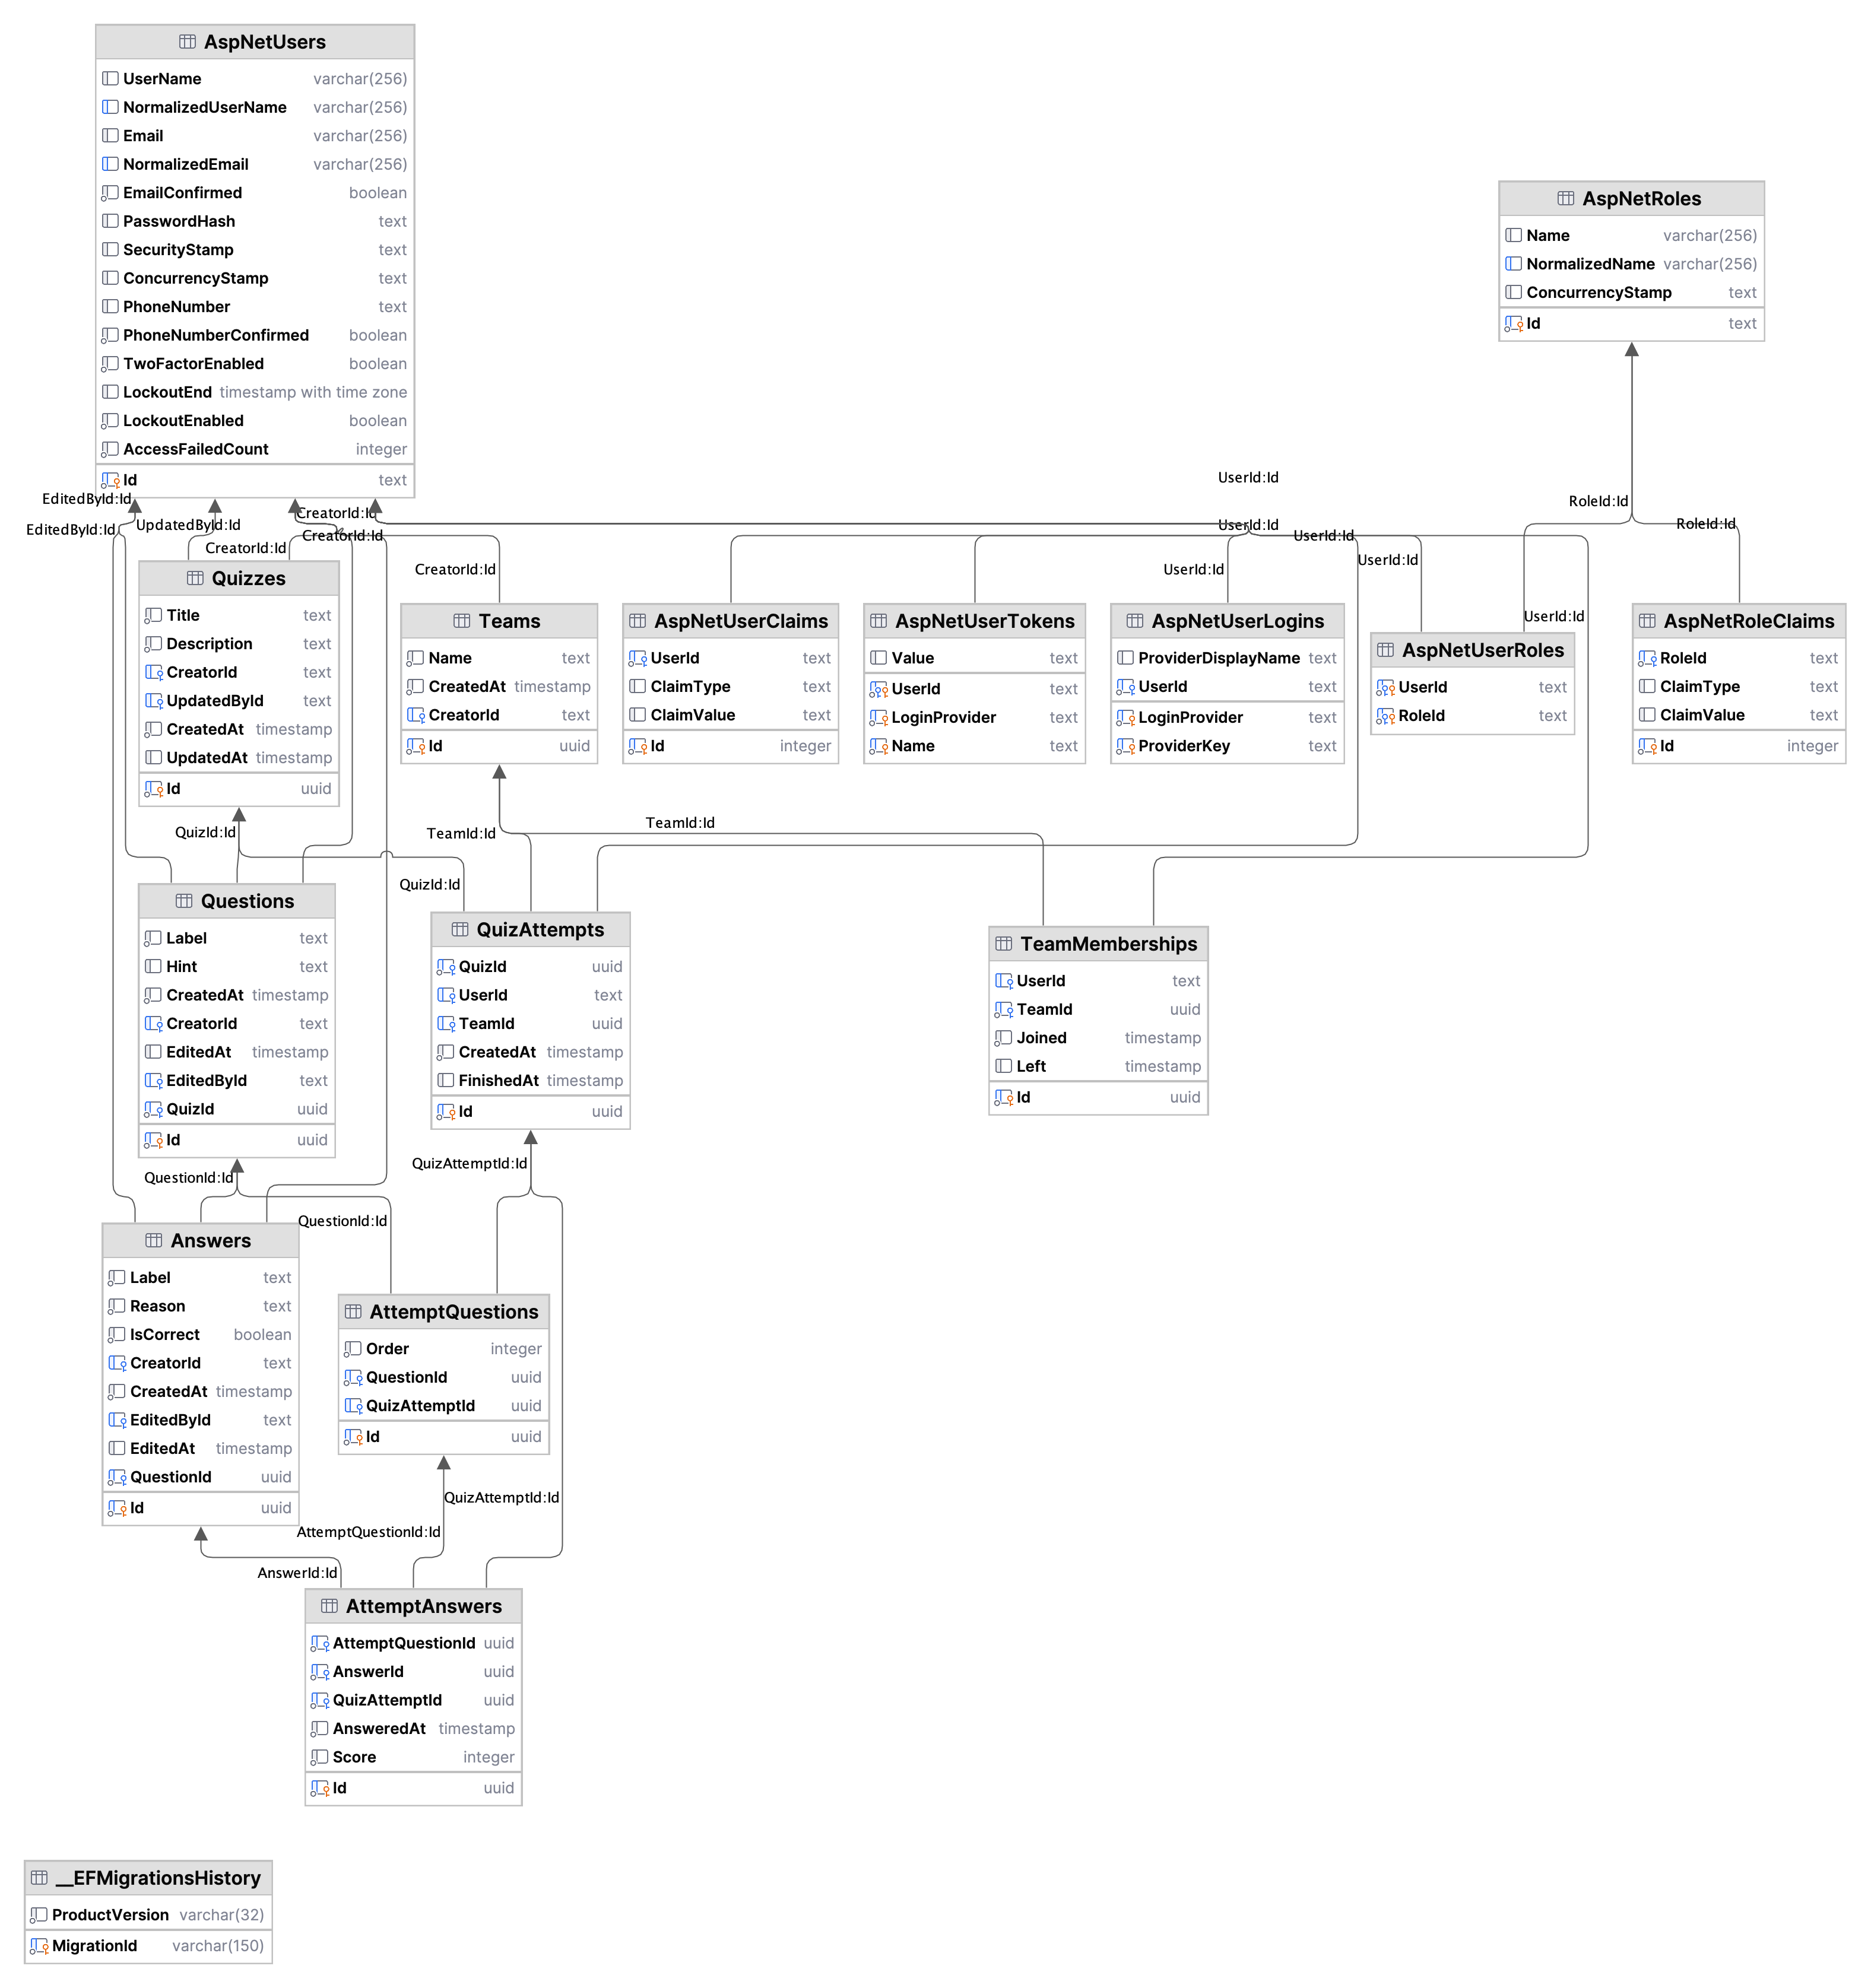
\includegraphics[width=0.9\textwidth]{img/ERD-Diagramm.png}
  \caption{Entity Relationship Diagramm}
\end{figure}

\noindent In dem ERD-Diagramm ist zu erkennen, dass die Datenbank-Modelle eine ähnliche Struktur wie die Backend-Modelle aufweisen.
Dies ist darauf zurückzuführen, dass das Entity Framework die Datenbank-Modelle automatisch aus den Backend-Modellen generiert. 
Jedoch wurden die Properties, welche eigene Klassen darstellen in Tabellen umgewandelt und über 'Foreign Keys' verknüpft. \newline

\noindent Die Tabelle '\_EFMigrationHistory' in ERD-Diagramm wird vom Entity Framework automatisch generiert und dient zur Verwaltung der Migrationen.
Migrationen sind Änderungen an der Datenbankstruktur, die vom Entity Framework automatisch durchgeführt werden, wenn sich bei der Entwicklung
Backend-Models ändern. \newline

\noindent Die Tabelle 'AspNetUsers' im ERD-Diagramm wird vom ASP.NET Identity Framework automatisch generiert und dient zur Verwaltung der Benutzer.
Außerdem wurden die Tabellen 'AspNetUserClaims', 'AspNetUserLogins' und 'AspNetUserRoles' auch von ASP.NET Identity Framework generiert.

\subsubsection{API Modelle}

In .NET werden häufig sogenannte DTOs (Data Transfer Objects) 
zur Definition von API-Modellen verwendet. Diese DTOs können sich von den Datenbankmodellen 
unterscheiden und sind speziell an die Anforderungen der API angepasst. 
Die Verwendung von DTOs bietet eine Reihe von Vorteilen:

\begin{itemize}
  \item \textbf{Verschleierung der Datenbankstruktur:} Die Verwendung von DTOs ermöglicht die Verschleierung der Datenbankstruktur
   gegenüber externen Parteien. Dies geschieht, indem nur die DTOs nach außen sichtbar sind. Wenn die Kommunikation
  über interne Backend-Modelle erfolgen würde und diese direkt über das Entity Framework in die Datenbank gespiegelt würden, 
  könnte eine externe Partei die Datenbankstruktur rekonstruieren. Durch die Verwendung von DTOs bleibt die Datenbankstruktur geschützt.
  \item \textbf{Flexibilität \& Anpassbarkeit:} Die Verwendung von DTOs ermöglicht es, die API-Schnittstelle anzupassen, 
  ohne die Struktur des Projekts ändern zu müssen. Lediglich das Mapping zu den internen Modellen muss an die neuen Anforderungen 
  angepasst werden. Dies erleichtert die Aktualisierung der API, ohne dass umfangreiche Änderungen am gesamten Projekt vorgenommen 
  werden müssen.
  \item \textbf{Angepassbarkeit:} Durch die Verwendung von DTOs kann die API-Definition sehr präzise angepasst werden. 
  In vielen Fällen ist das Modell, das an das System gesendet wird, nicht identisch mit dem Modell, das das System zurückgibt. 
  Ein gutes Beispiel hierfür ist die Registrierung eines Benutzers. Bei der Registrierung wird ein Passwort an das System gesendet. 
  Wenn jedoch der Benutzer über die entsprechende Schnittstelle abgerufen wird, wird das Passwort nicht zurückgegeben. 
  Dies ermöglicht eine flexible Anpassung der API an die unterschiedlichen Anforderungen und Sicherheitsaspekte.
\end{itemize}

\subsection{Kommunikation zwischen Frontend und Backend}

Das Backend und das Frontend kommunizieren über das HTTP Protokoll und verwendet zur als interface eine API-Schnittstelle.
Im folgenden wird zuerst erklärt, wie diese Kommunikation funktioniert und wie diese Daten dann im Backend verarbeitet werden.

\subsubsection{Kommunikations Schnittstelle}

Die Kommunikation zwischen Backend und Frontend funktioniert über das HTTP Protokoll.
Dabei gehen die Anfragen immer vom Client and den Server. Der Server Antwortet entsprechend zu der Anfrage.
Im generellen unterscheidet man zwischen 4 verschiedene requests. Diese Request Typen sind wie folgt:

\begin{itemize}
\item \textbf{GET-Requests:} Diese Requests werden verwendet um Daten abzurufen.
\item \textbf{POST-Request:} Dieser Request-Typ wird verwendet um neue Dinge anzulegen.
\item \textbf{PUT-Requests:} Dieser Request-Typ wird genutzt um Elemente upzudaten
\item \textbf{PATCH-Requests:}
\item \textbf{DELETE-Requests:} Diese Request-Typ wird verwendet um Elemente zu löschen.
\end{itemize}

\noindent Die Request Methode steht im Header der HTTP Anfrage. Über diese Methoden ist es mögliche einen
API Pfad mehrfach zu belegen. \newline

\noindent Der REST-Standart beschreibt wie man API Schnittstellen logisch und nachvollziebar aufbauen muss.
Dabei werden Pfad Pattern aber auch Request-Typen vorgeschrieben. Nach diesem REST-Standard haben wir die API
für das Quiz Projekt erstellt. Dies ist vor allem im Bezug auf wartbarkeit sehr wichtig. Außerdem ermöglicht
eine klare API Schnittstellen Definition, dass andere Entwickler andere Oberfläche für unsere API Schnittstelle bauen können (Mobile APPs).

\subsubsection{API-Schnittstellen}

\begin{figure}[H]
  \centering
  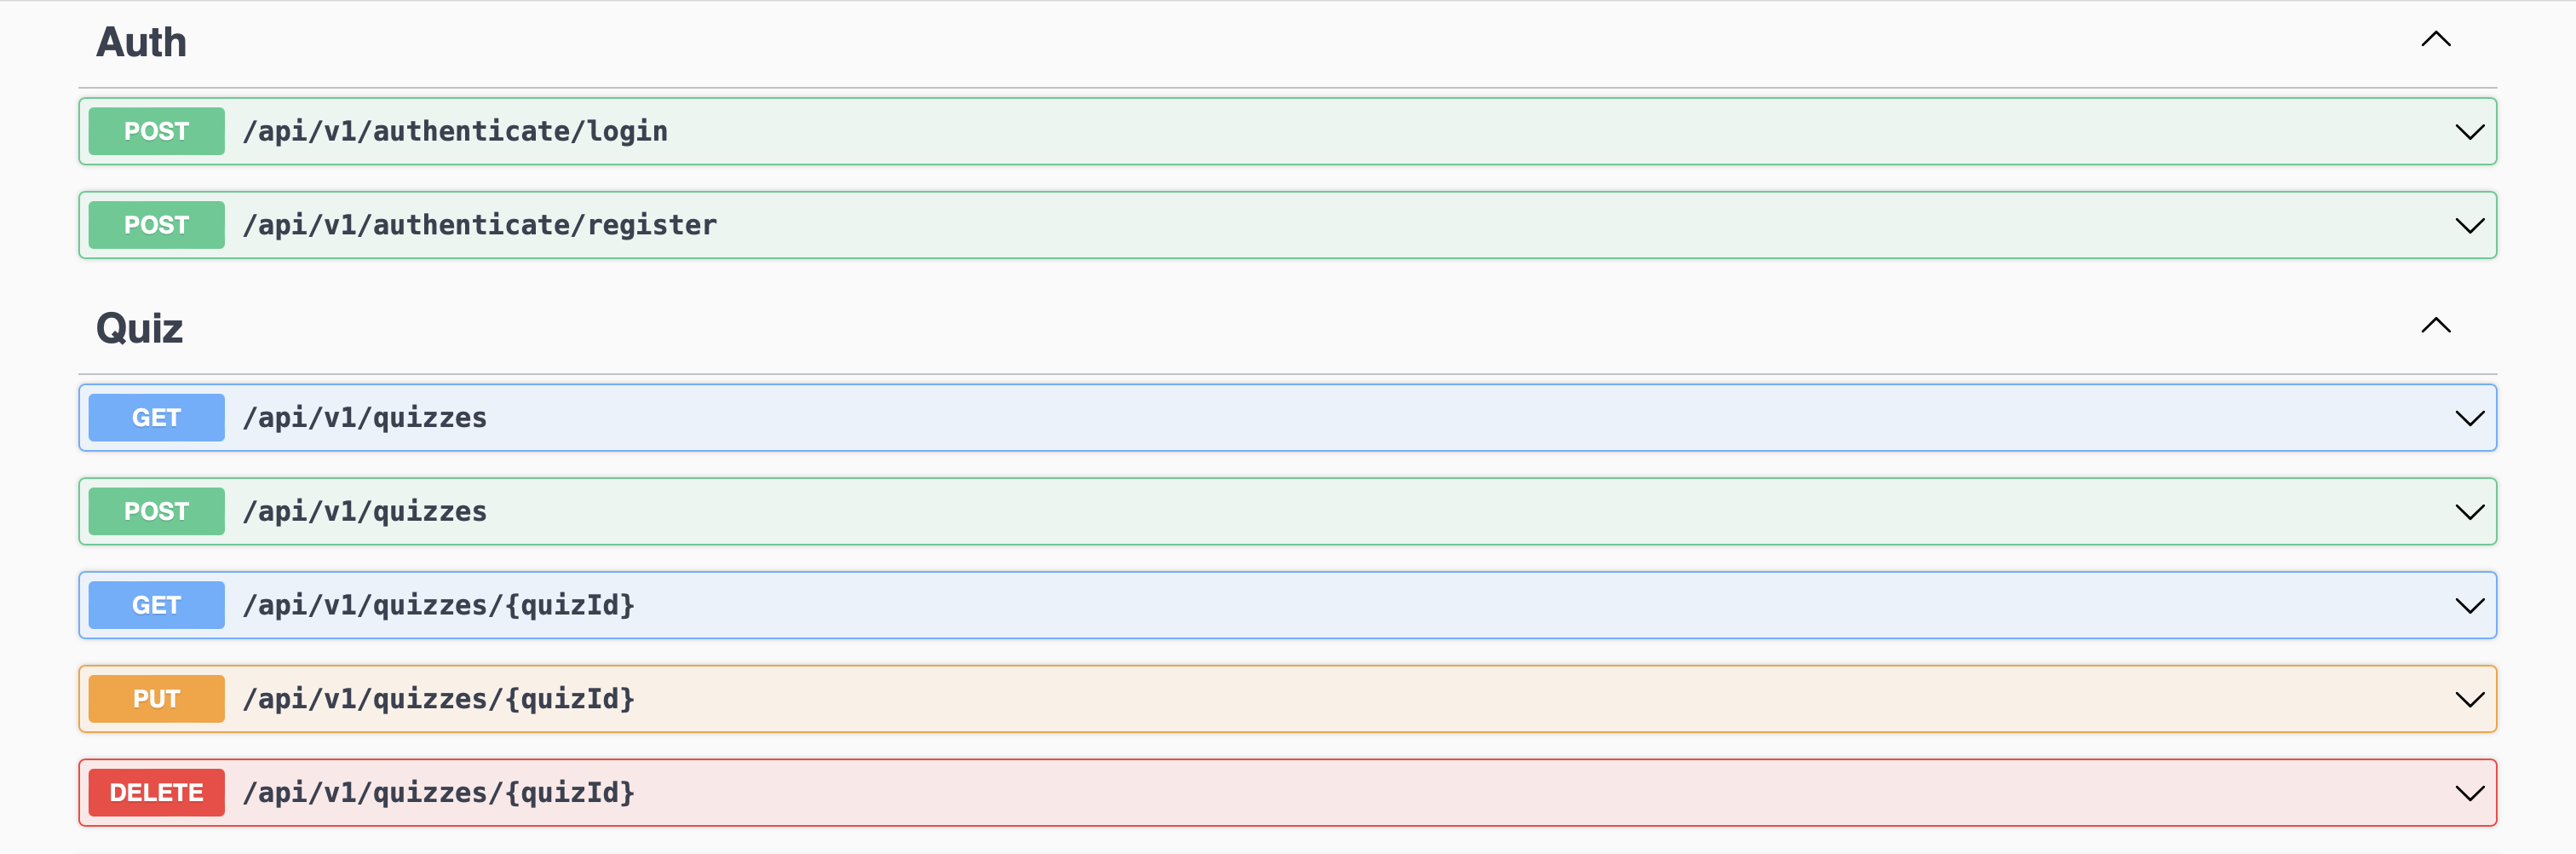
\includegraphics[width=0.9\textwidth]{img/Auth_Quiz-Endpoint.png}
  \caption{Auth \& Quiz API Endpoint Definition}
\end{figure}


\begin{figure}[H]
  \centering
  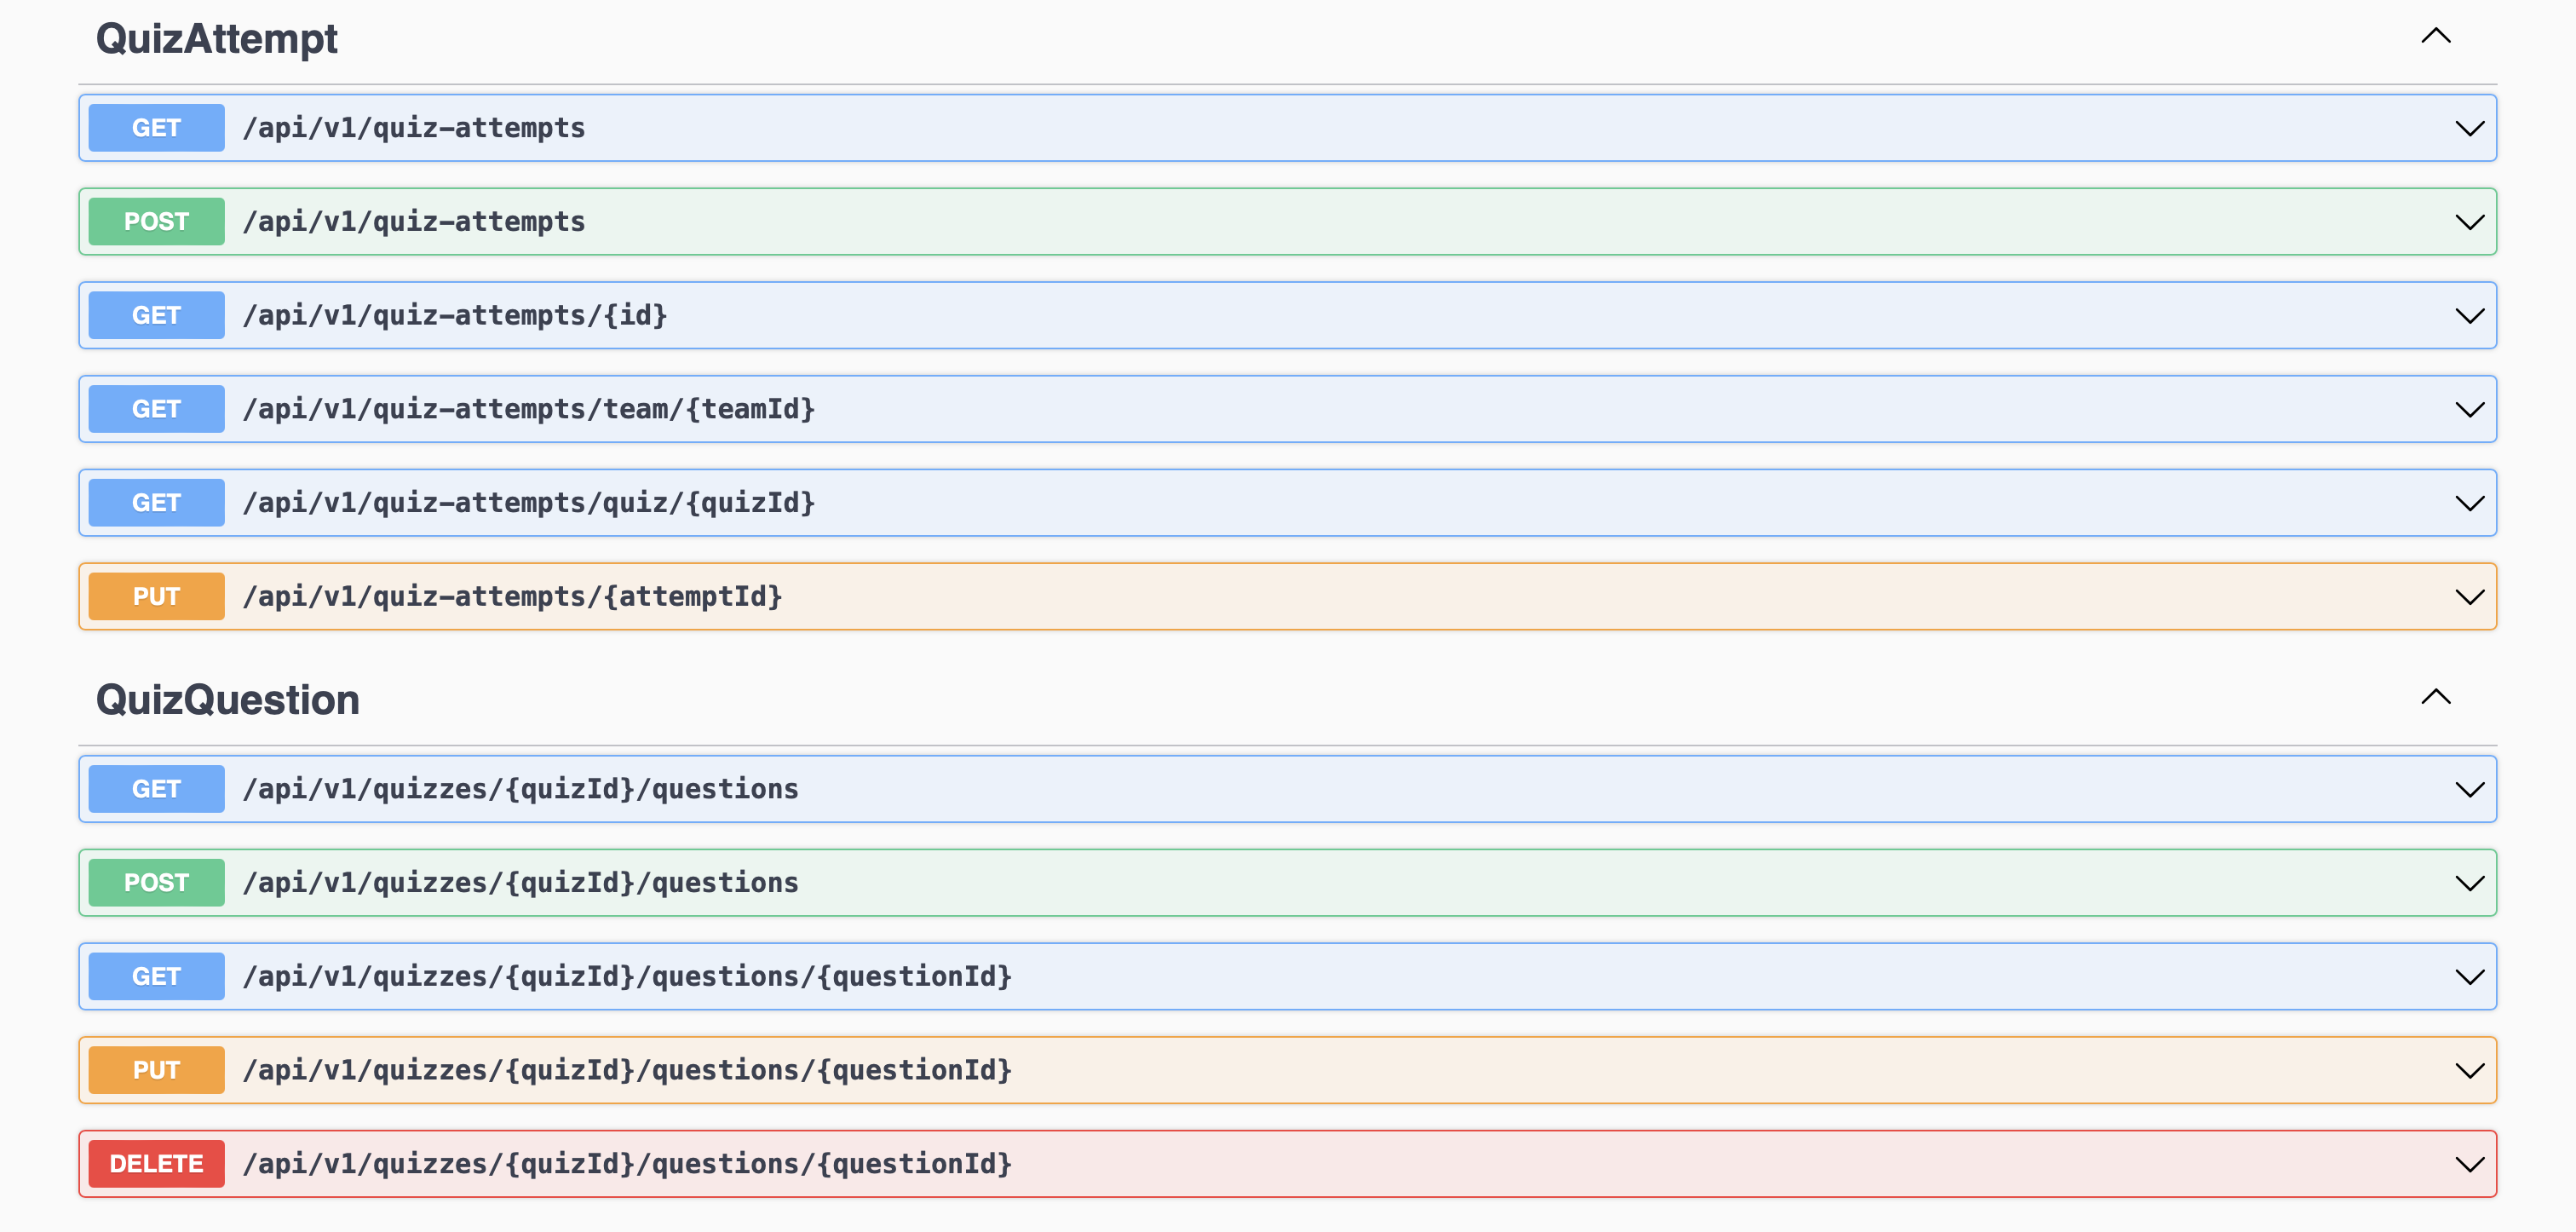
\includegraphics[width=0.9\textwidth]{img/QuizAttempt_QuizQuestion-Endpoint.png}
  \caption{Quiz Attempt \& Quiz Question Endpoint Definition}
\end{figure}



\begin{figure}[H]
  \centering
  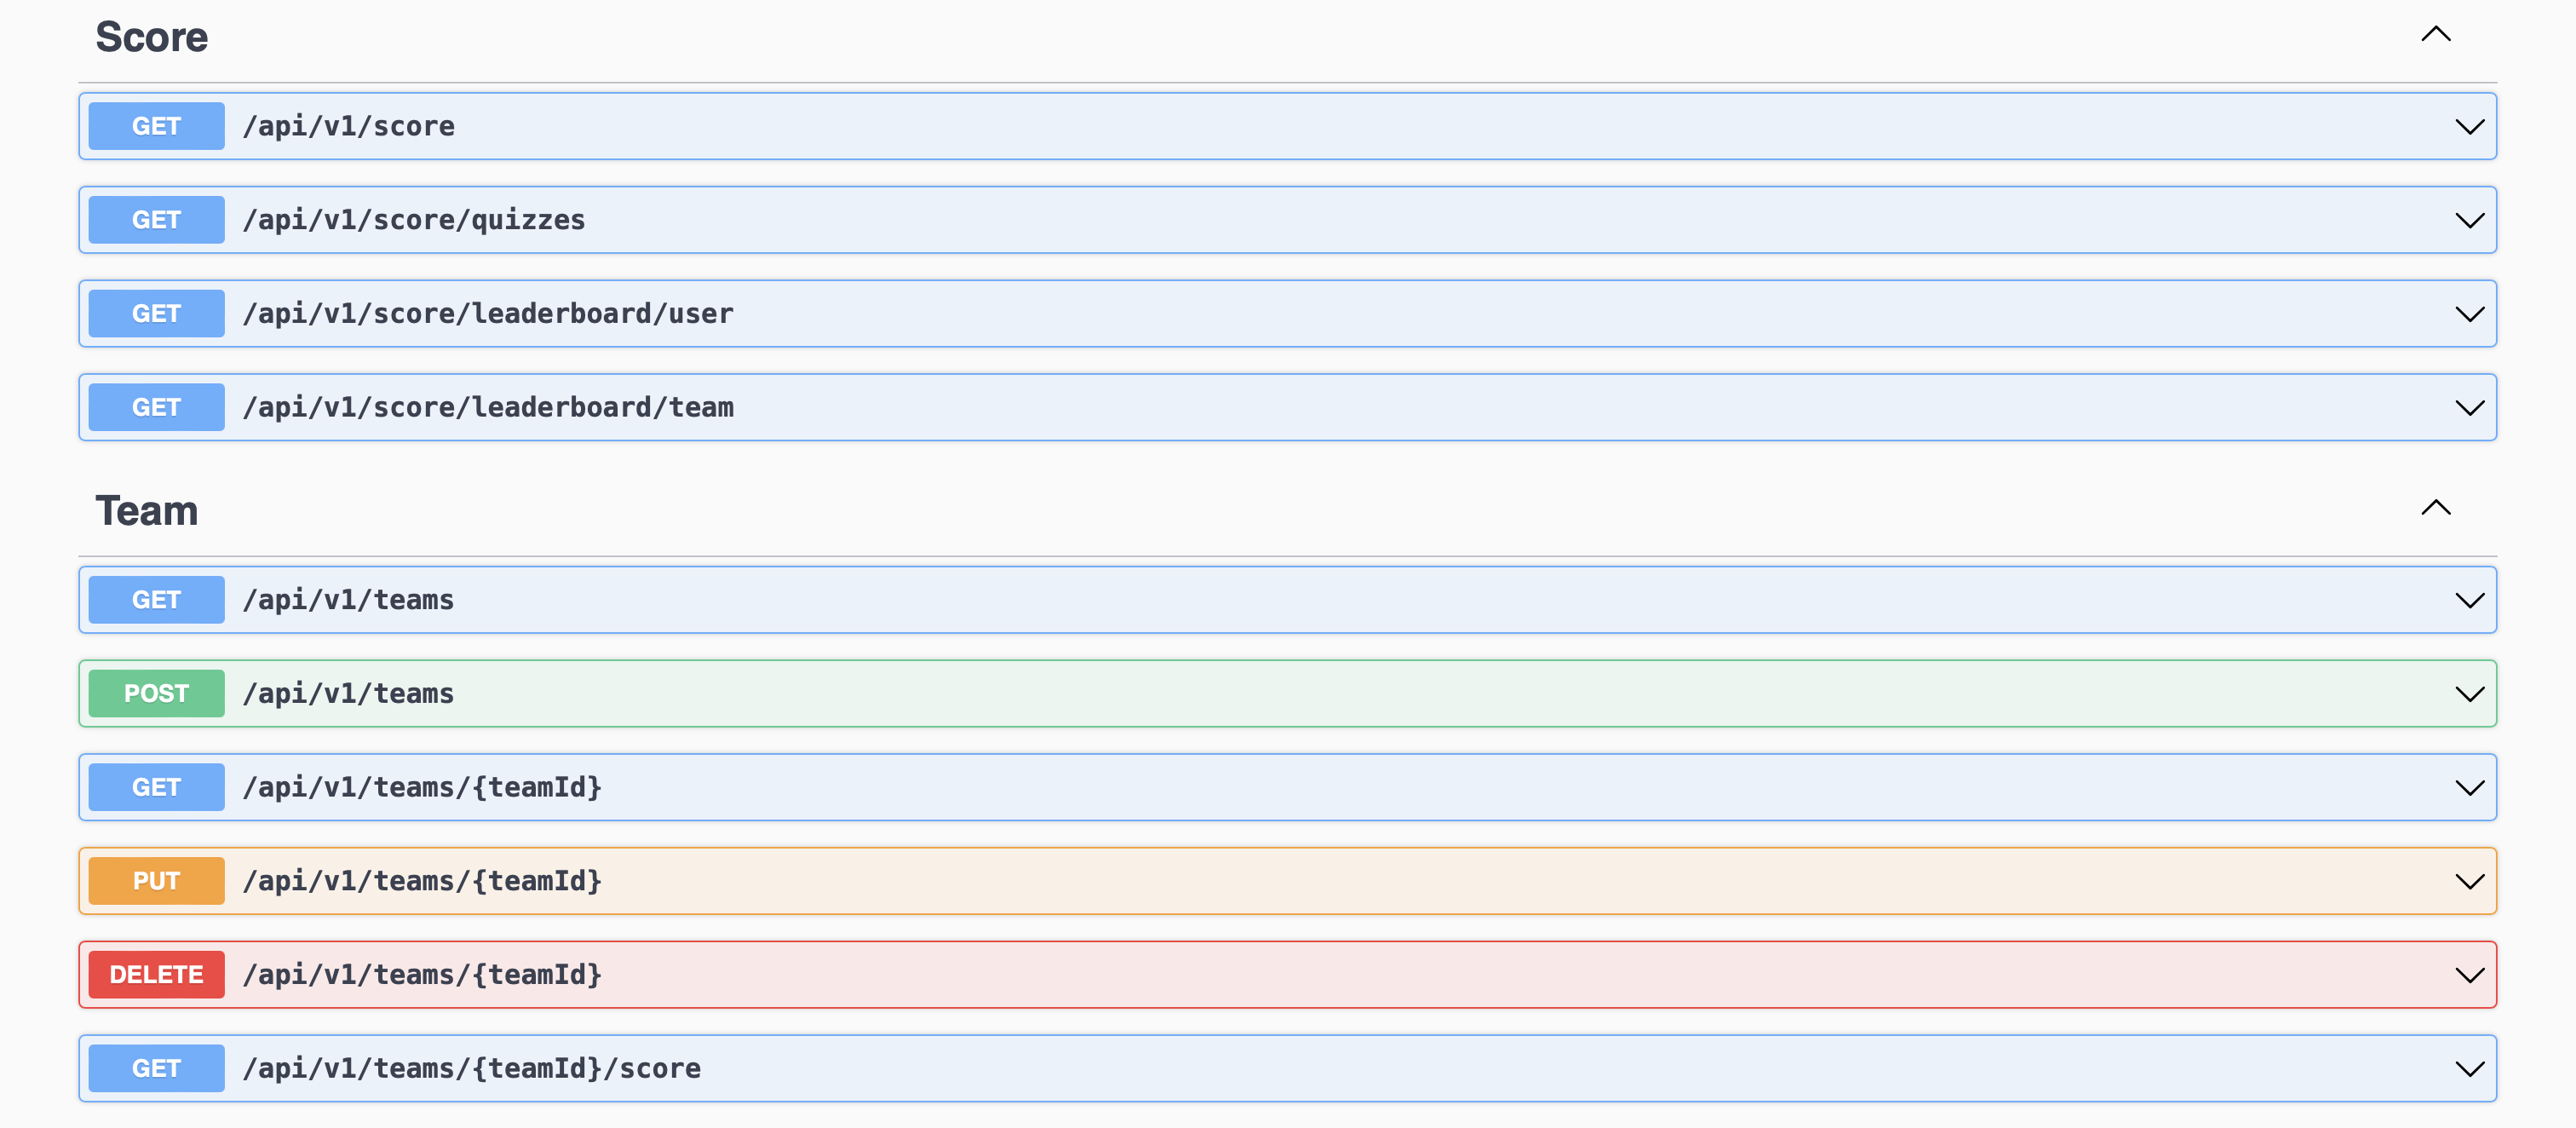
\includegraphics[width=0.9\textwidth]{img/Score_Team-Endpoint.png}
  \caption{User \& Score API Endpoint Definition}
\end{figure}


\begin{figure}[H]
  \centering
  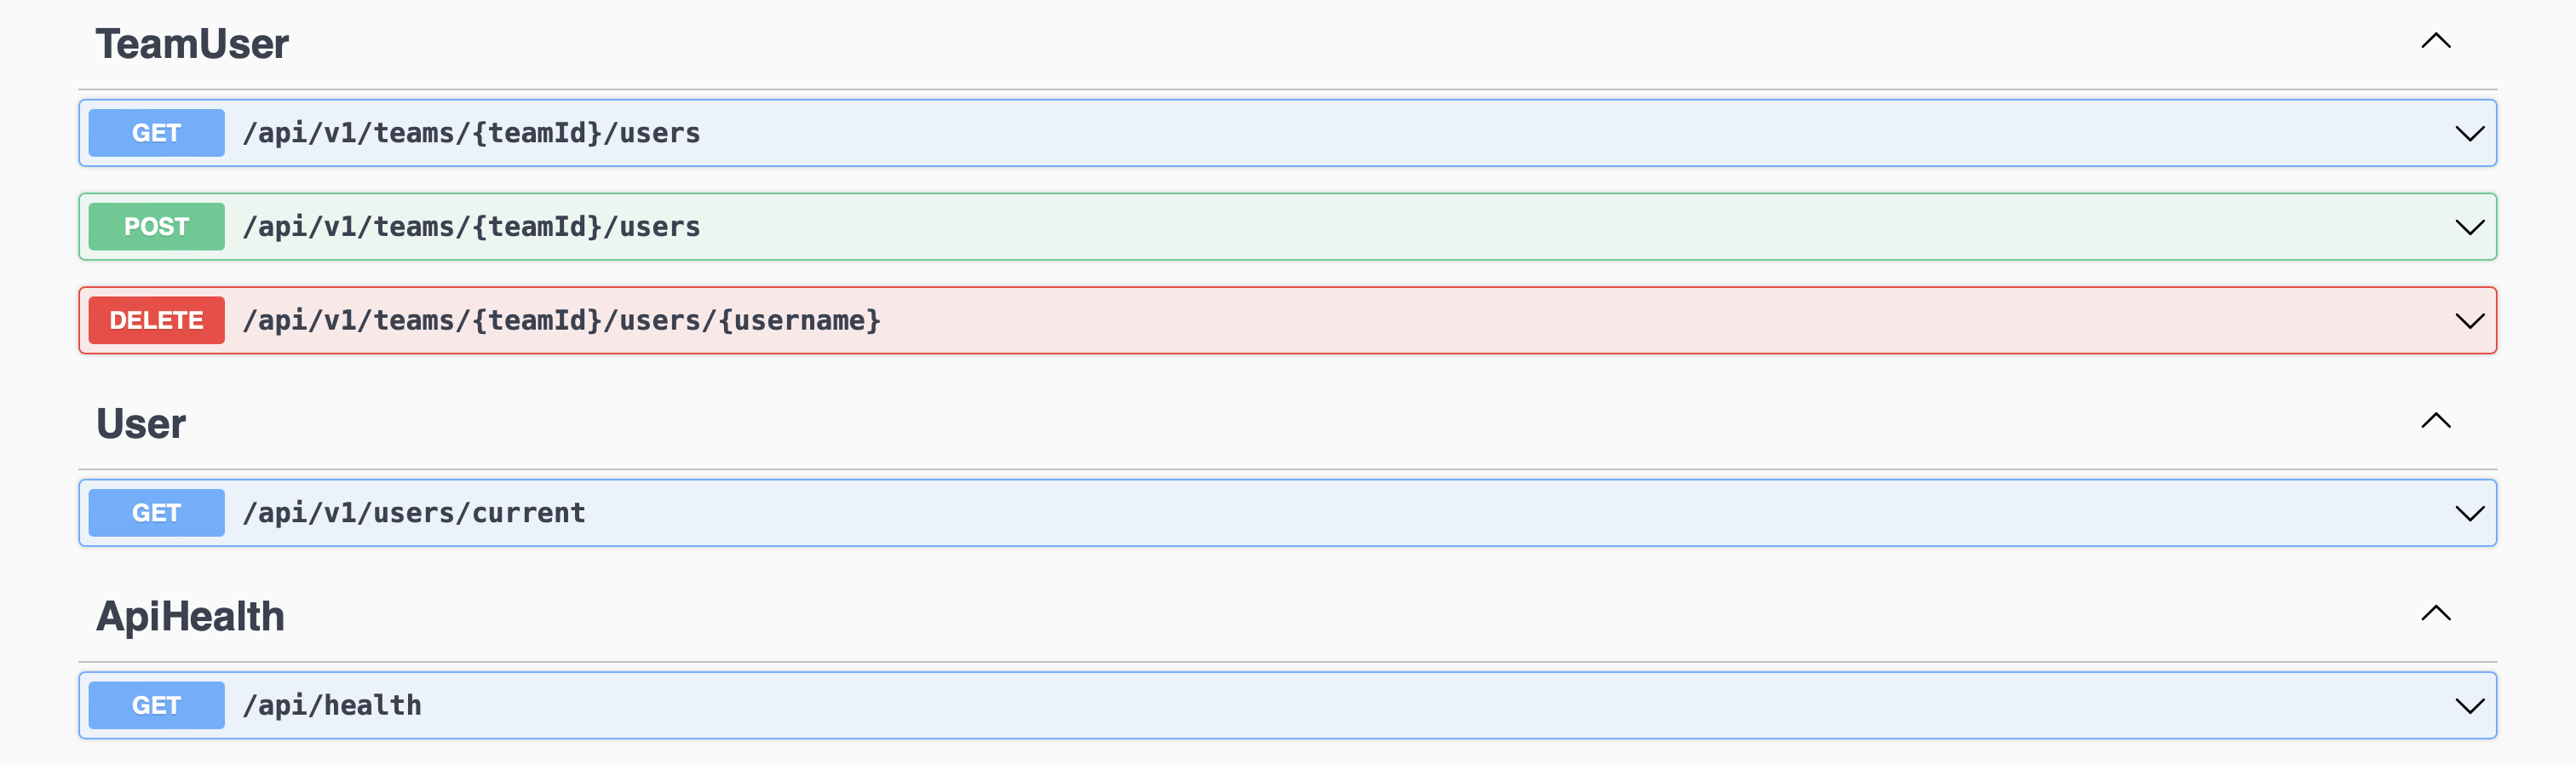
\includegraphics[width=0.9\textwidth]{img/TeamUser_User-Endpoint.png}
  \caption{Team \& Team-User API Endpoint Definition}
\end{figure}

\subsubsection{Datenflow im Backend}

\begin{figure}[H]
  \centering
  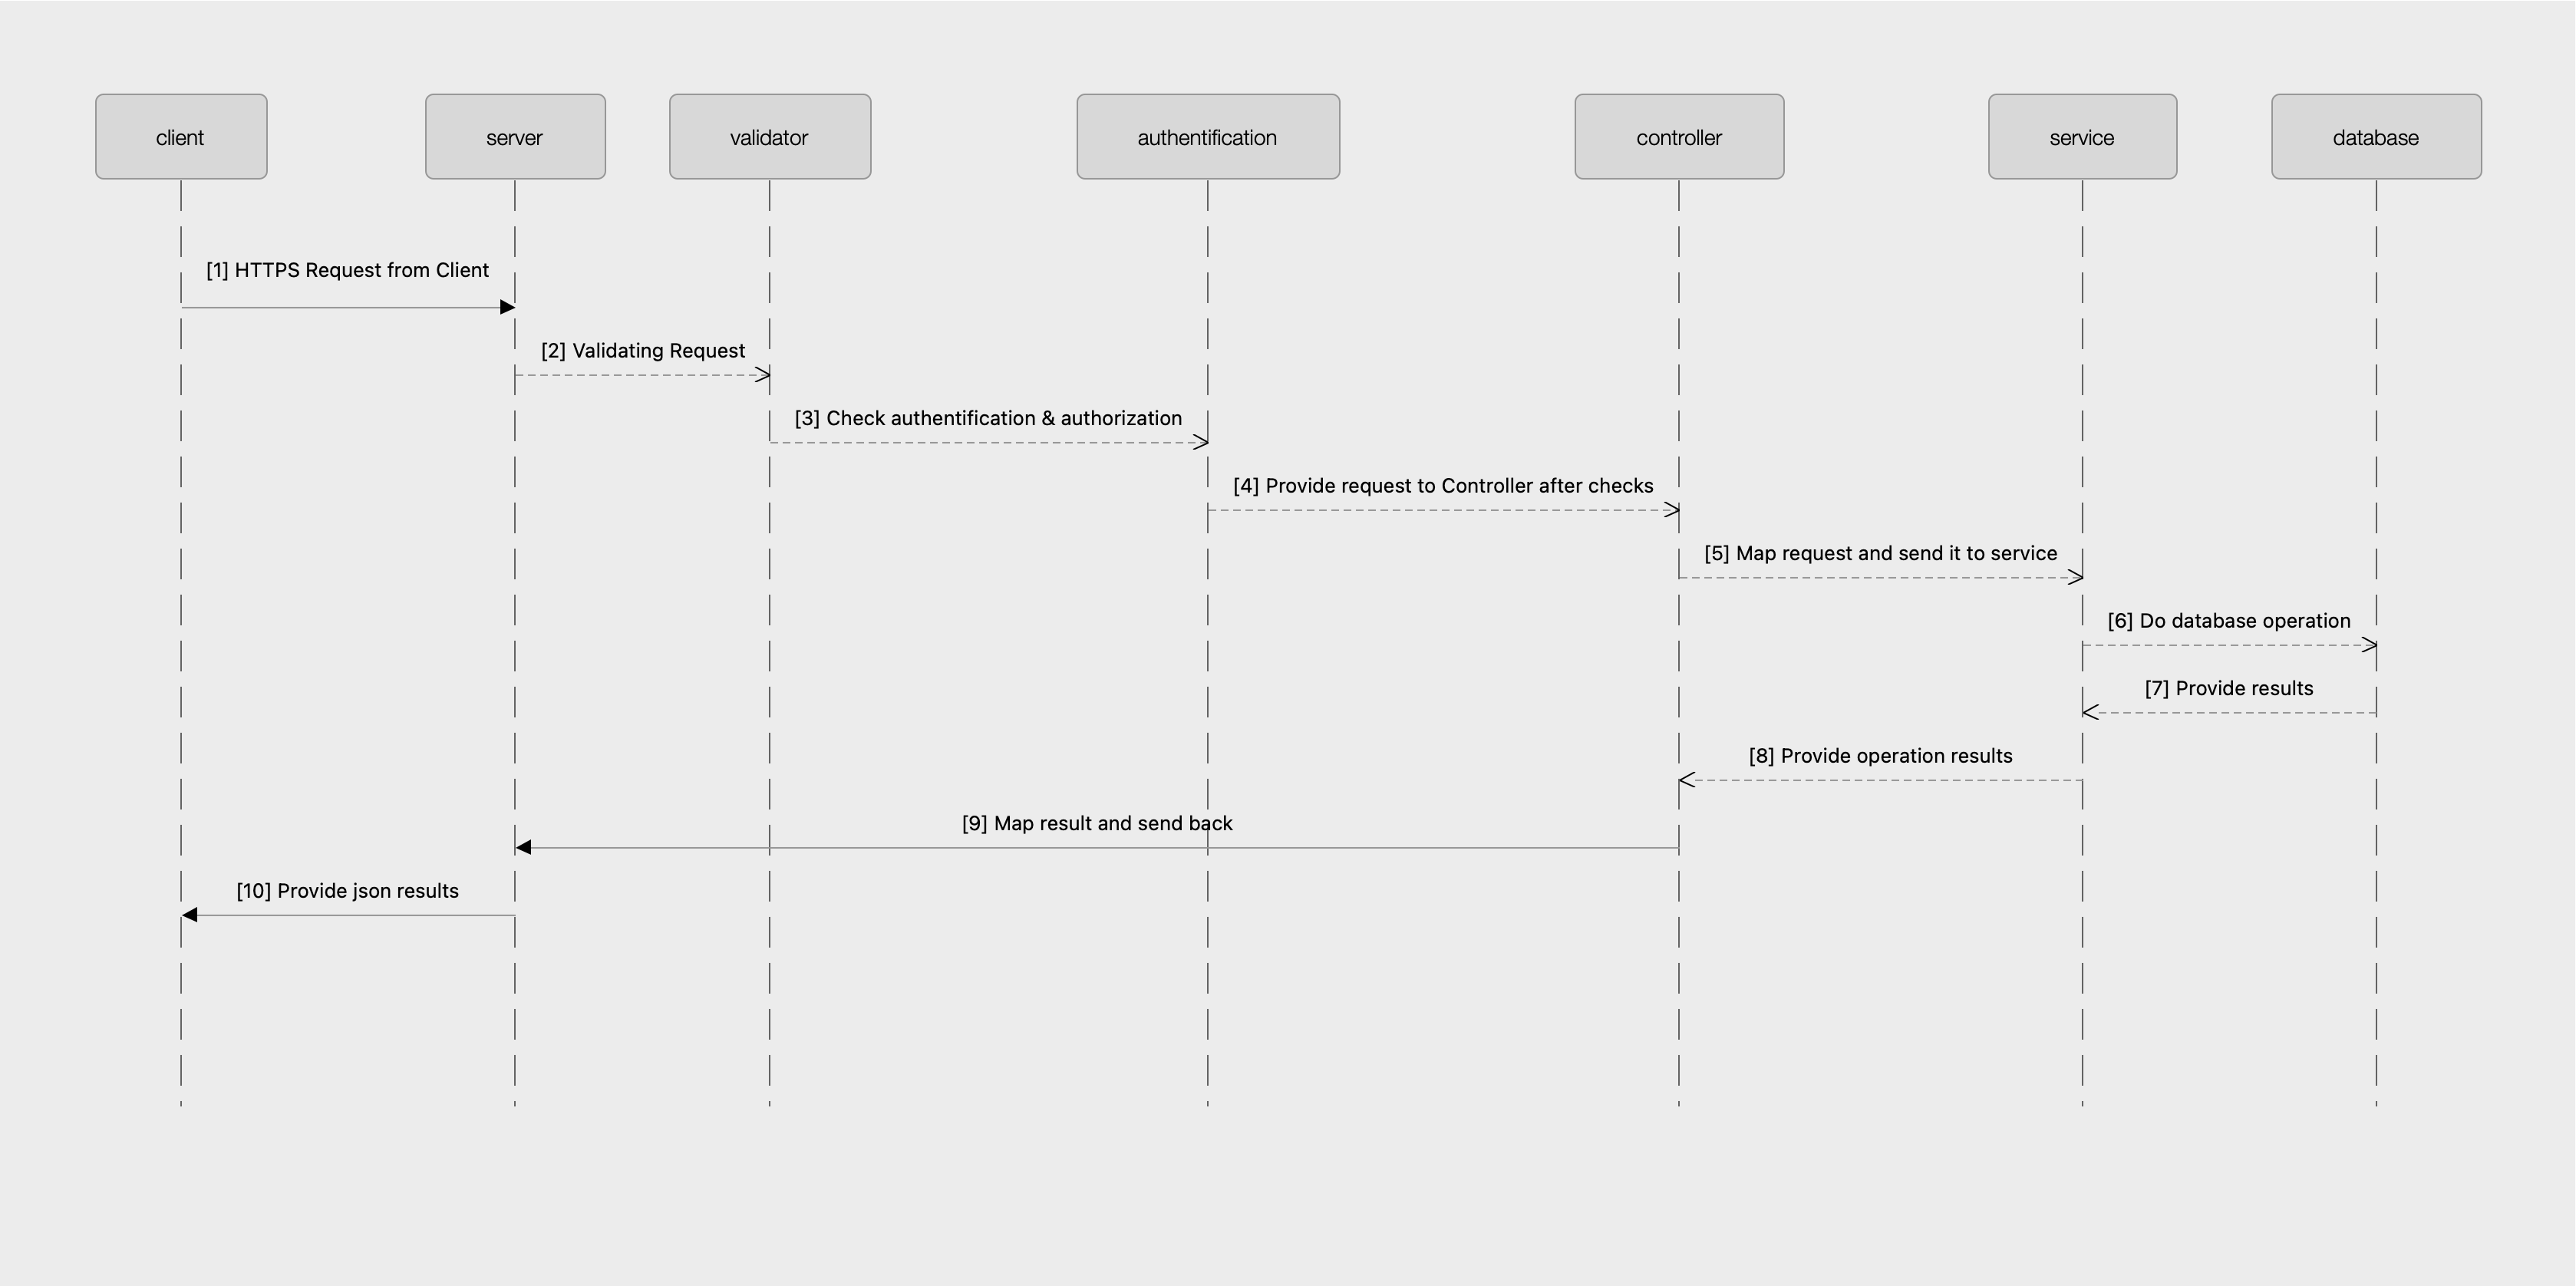
\includegraphics[width=0.9\textwidth]{img/Backend-Flow.png}
  \caption{Flow Diagramm API Request}
\end{figure}

